% instead of amberg, the option weiden oder amwen can be given. This changes the title backround
% lecture argument adds the subtitle to the footline
% other formats possible, e.g. aspectratio=43 or aspectration=169
\documentclass[aspectratio=169, lecture, amberg]{OTHAWbeamer}
\let\Tiny=\tiny

\usepackage{etex}
\usepackage{array}
\usepackage{booktabs}
\usepackage{graphicx}
\usepackage{hyperref}
\usepackage[utf8]{inputenc}
\usepackage[english]{babel}
\usepackage{amsmath}
\usepackage[
backend=biber,
style=ieee,
sorting=none
]{biblatex}

\title[Kurztitel]{AI Conference}
\subtitle{Exploring Semantic Consistency in Unpaired Image Translation to Generate Data for Surgical Applications}
\author[Mustermann]{Vinay Kumar}
\place{Amberg}
\date{{\selectlanguage{english}\today}}

\addbibresource{literature.bib}

% Customize Table of Contents appearance
\setbeamertemplate{section in toc}[sections numbered]
\setbeamertemplate{subsection in toc}[subsections numbered]

\begin{document}
\maketitle

% Table of Contents slide
\begin{frame}{Table of Contents}
    \tableofcontents
\end{frame}

% Sections are added here to appear in the Table of Contents
\section{Introduction and Motivation}
\section{Methodology and Experiments}

\section{Evaluation and Results}
\section{Purpose and Contribution}
\section{Summary and Conclusion}


\begin{frame}
    \frametitle{Introduction and Motivation}
    \framesubtitle{Introduction of the Topic}
    Exploring Semantic Consistency in Unpaired Image Translation to Generate Data for Surgical Applications.
    \begin{itemize}
        \item \textbf{Semantic Consistency}: keeping the important details and meaning of the original image the same when it is changed or translated into another type of image.  
    \end{itemize}

    \begin{figure}
        \centering
        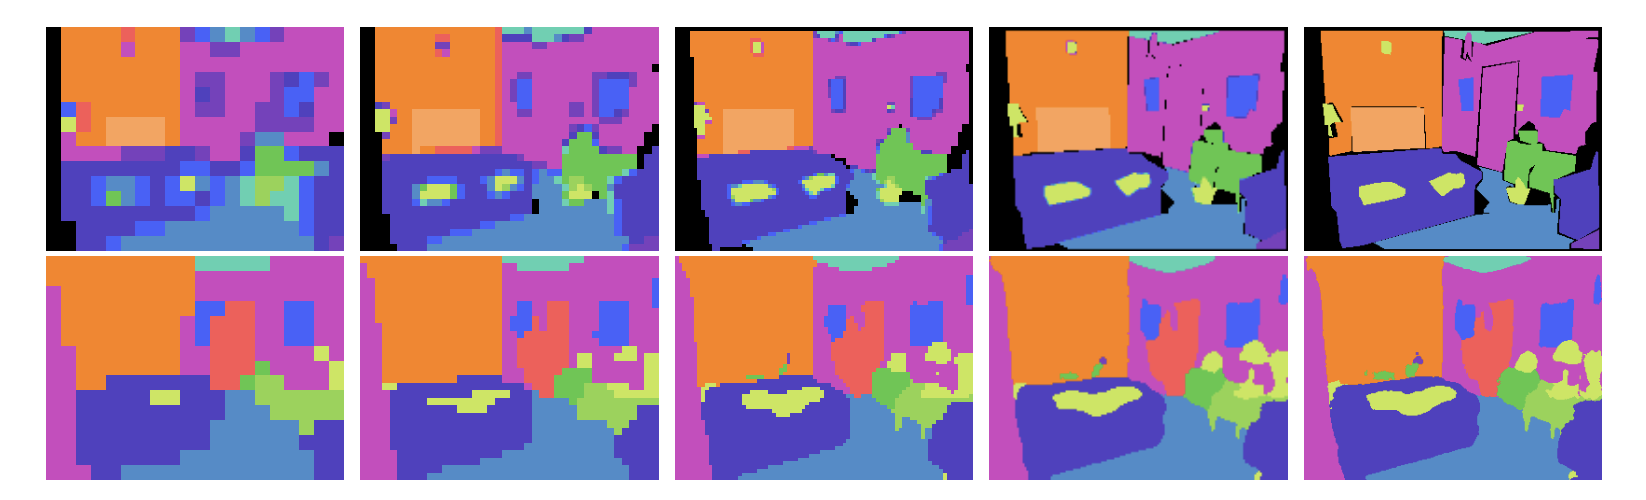
\includegraphics[width=0.8\linewidth]{semantic.png}
        \caption{\cite{https://cvg.cit.tum.de/_media/spezial/bib/lingni17iros.pdf}}
    \end{figure}

  \end{frame}


  \begin{frame}
    \frametitle{Introduction and Motivation}
    \framesubtitle{Introduction of the Topic}
    
    \begin{itemize}
        \item \textbf{Unpaired Image}: Unpaired images are sets of images from different domains that do not have a direct relation between them
    \end{itemize}
    
    \begin{figure}
        \centering
        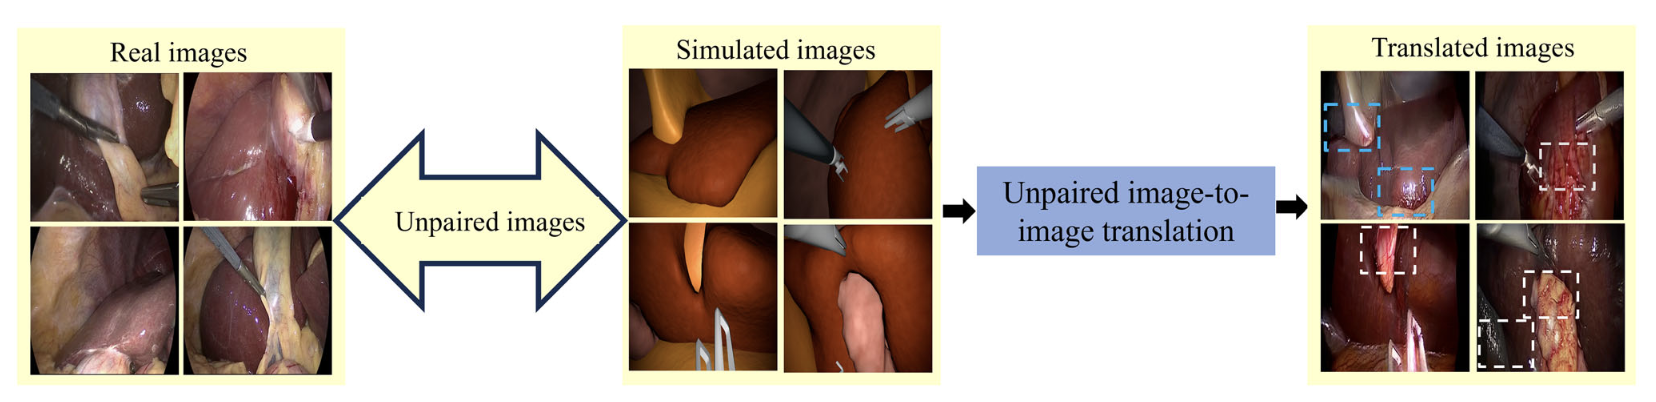
\includegraphics[width=0.9\linewidth]{unpaired.png}
        
    \end{figure}
    
\end{frame}



  \begin{frame}
    \frametitle{Introduction and Motivation}
    \framesubtitle{Introduction of the Topic}
    \begin{itemize}
         \item \textbf{Generating Data}
         \begin{itemize}
            \item refers to creating new images by translating synthetic images into realistic ones using techniques like unpaired image-to-image translation.
            \item helps produce large, labeled datasets needed for training models, especially when collecting real data is challenging
         \end{itemize}

    \end{itemize}
    \begin{figure}
        \centering
        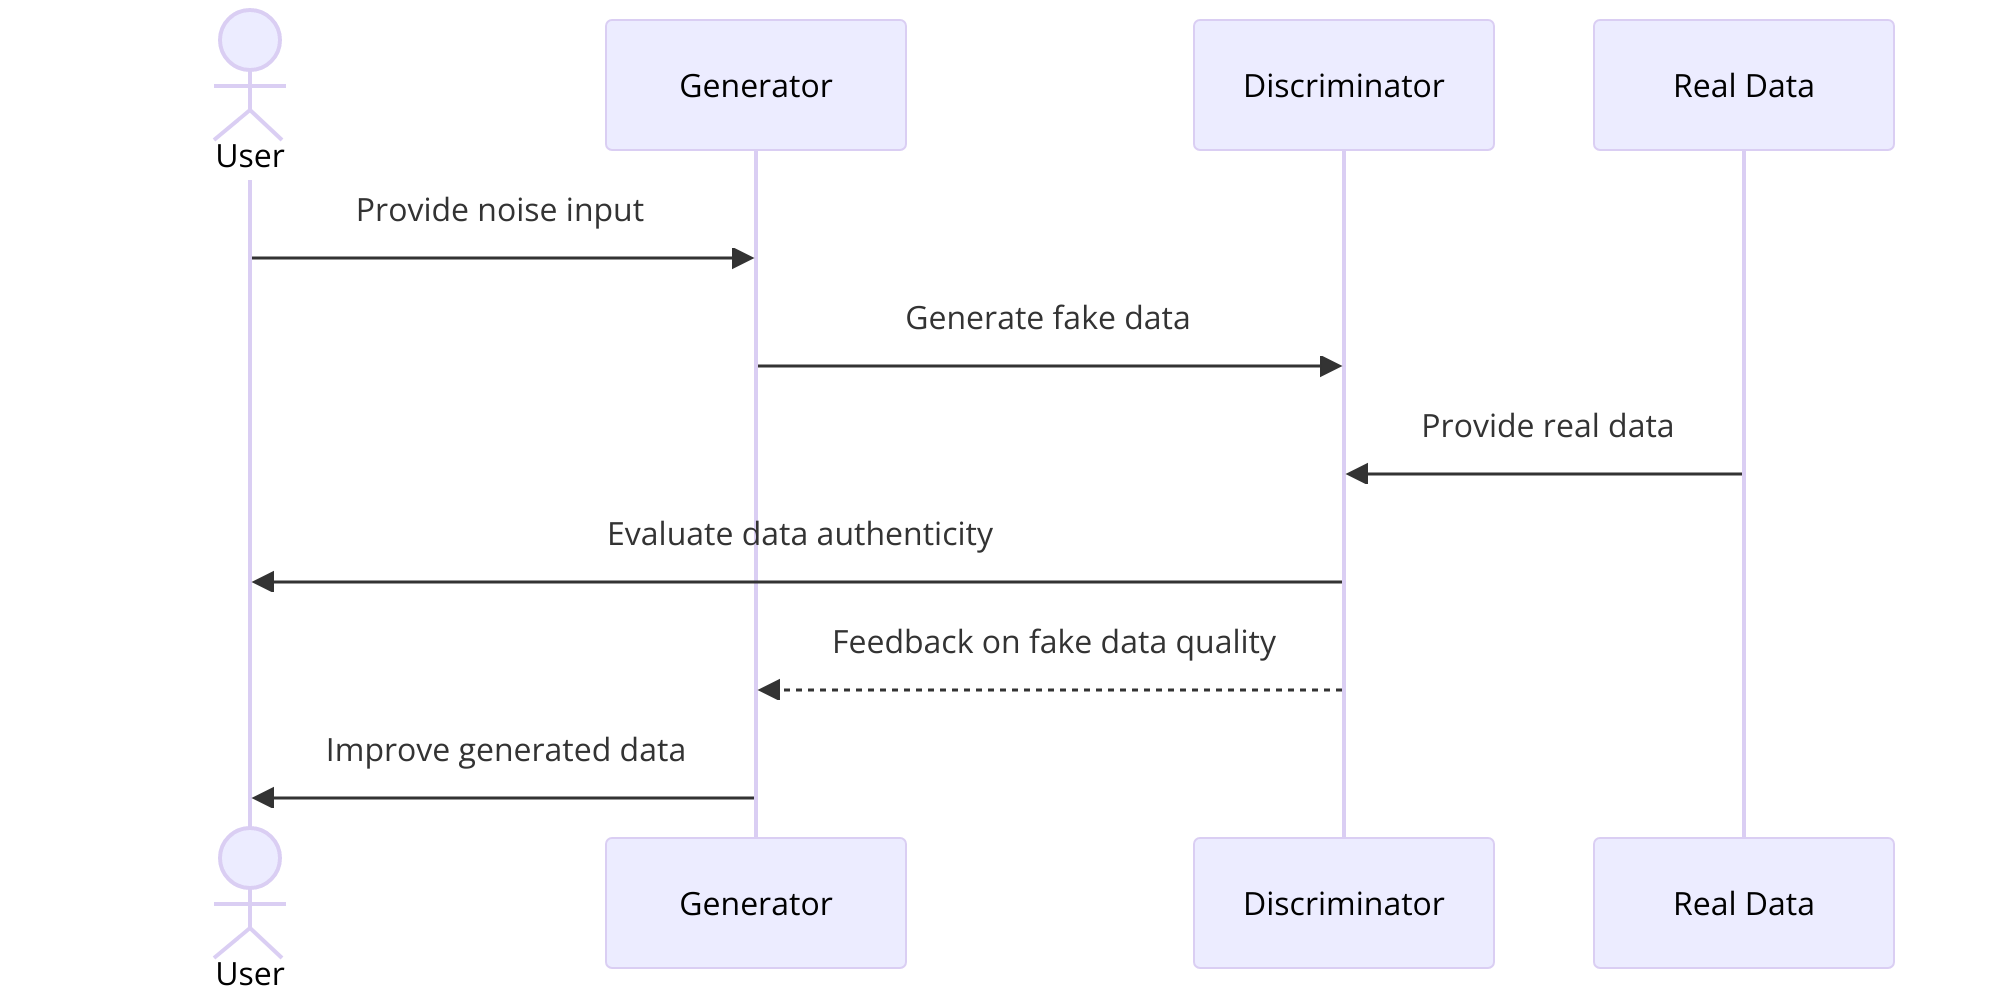
\includegraphics[width=0.55\linewidth]{diagram.png} % Adjust the width as needed
        % \caption{\cite{AI Generated}}
    \end{figure}
  \end{frame}

  \begin{frame}
    \frametitle{Introduction and Motivation}
    \framesubtitle{Introduction of the Topic}
    
    \begin{columns}[T] % align columns to the top
        \begin{column}{0.5\textwidth}
            \textbf{Historical Knowledge}
            \begin{itemize}
                \item Evolution of Medical Image Analysis
                \vspace{0.4cm}
                \item Impact of AI and Deep Learning
                \vspace{0.4cm}
                \item Need for Large Annotated Datasets
                \vspace{0.4cm}
                \item Shift Towards Automation
            \end{itemize}
        \end{column}
        
        \begin{column}{0.52\textwidth}
            \begin{figure}
                \centering
                \hspace*{-1cm}
                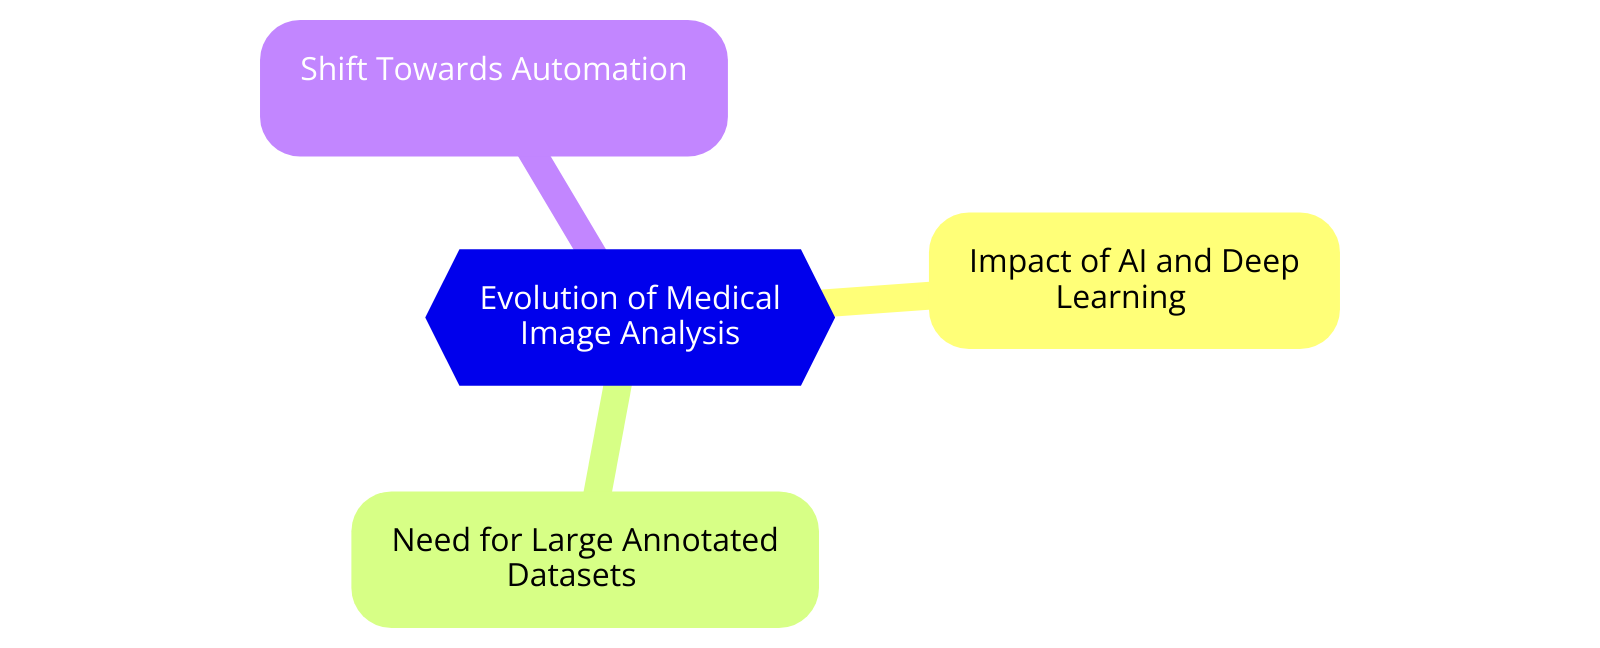
\includegraphics[width=1.3\linewidth]{AI_evolution.png} % Adjust the width as needed
                % \caption{\cite{AI Generated}}
            \end{figure}
        \end{column}
    \end{columns}
    
\end{frame}

  \begin{frame}[t]
    \frametitle{Introduction and Motivation}
    \framesubtitle{Introduction of the Topic}
    
    \vspace{0.2cm} % Adjust this value as needed to move the content upwards
    \begin{itemize}
        \item \textbf{Key Concepts}
         \vspace{0.4cm}
        \begin{itemize}
            \item Image-to-Image Translation
            \vspace{0.4cm}
            \item Unpaired Image Translation
            \vspace{0.4cm}
            \item Semantic Consistency
            \vspace{0.4cm}
            \item Generative Adversarial Networks (GANs)
            \vspace{0.4cm}
            \item Contrastive Learning
        \end{itemize}
    \end{itemize}
    
\end{frame}

\begin{frame}[t]
    \frametitle{Introduction and Motivation}
    \framesubtitle{Introduction of the Topic}
    
    \vspace{0.2cm} % Adjust this value as needed to move the content upwards
    \begin{itemize}
        \item \textbf{Limitation of Current Literature}
        \vspace{0.4cm}
        \begin{itemize}
            \item Scarcity of Annotated Data
            \vspace{0.4cm}
            \item Challenges in Semantic Consistency
            \vspace{0.4cm}
            \item Limitations of Paired Image Translation
            \vspace{0.4cm}
            \item Failure in Handling of Real-World Medical Imaging
        \end{itemize}
    \end{itemize}

    \begin{block}{Note}
        Despite its advancements, this study does not address the synthesis of multi-modal data or ensure temporal consistency in video datasets, which remain areas for future exploration.
        \end{block}
    
\end{frame}

\begin{frame}[t]
    \frametitle{Introduction and Motivation}
    \framesubtitle{Introduction of the Topic}
    
    \vspace{0.2cm} % Adjust this value as needed to move the content upwards
    \begin{itemize}
        \item \textbf{Importance of this Literature}
        \vspace{0.4cm}
        \begin{itemize}
            \item Addressing Data Scarcity with Synthetic Data
             \vspace{0.4cm}
            \item Enhancing Semantic Consistency
            \vspace{0.4cm}
            \item Unpaired Image Translation for Medical Imaging
            \vspace{0.4cm}
            \item Improving Real-World Applicability
        \end{itemize}
    \end{itemize}

    \begin{block}{Note}
        This study is crucial as it addresses the challenges of data scarcity and semantic consistency in medical imaging, providing a novel approach to generating high-quality annotated datasets from synthetic images. 
         \end{block}
    
\end{frame}

\begin{frame}[t]
    \frametitle{Introduction and Motivation}
    \framesubtitle{Introduction of the Topic}
    
    \vspace{0.1cm} % Adjust this value as needed to move the content upwards
    \textbf{Significance of this study}
    \begin{itemize}
        
            \item This paper proposes a ConStructS method, which combines contrastive learning and multi-scale structural similarity to solve the semantic consistency problem in unpaired image translation. It also include:
            \vspace{0.3cm}
        \begin{itemize}
            \item Improved Data Generation
            \vspace{0.4cm}
            \item Enhanced Semantic Consistency
            \vspace{0.4cm}
            \item Feasibility of Unpaired Image Translation
            \vspace{0.4cm}
            \item Real-World Applicability
            
            
        \end{itemize}
    \end{itemize}
    
\end{frame}

    
\begin{frame}[t]
    \frametitle{Methodology (Overall Approach)}
    \framesubtitle{Data Collection and Preparation}
    
    \begin{itemize}
        \item \textbf{Synthetic Data:} For this study, datasets resembling laparoscopic scenes were used\footnotemark[1]
        \item \textbf{Real Data:} Cholec80 dataset for cholecystectomy and a dataset of distal gastrectomy images\footnotemark[2]
        \item \textbf{Preprocessing:} Resizing, normalizing, and segmenting the images into relevant regions of interest (e.g., organs, surgical tools) to ensure compatibility with the model
    \end{itemize}
    
    \begin{block}{Note}
        In the dataset, approximately 26,000 images from 75 patients were used for training, and a separate segmentation dataset of 5 patients was chosen for evaluation
         \end{block}
    \vfill % Push the citations to the bottom of the frame
    \footnotetext[1]{\url{https://opencas.dkfz.de/image2image/}}
    \footnotetext[2]{\url{http://camma.u-strasbg.fr/datasets/}}
    
\end{frame}


\begin{frame}
    \frametitle{Methodology}
    \framesubtitle{Model Architecture}
    
    % Evaluation content here
    \begin{figure}
        \centering
        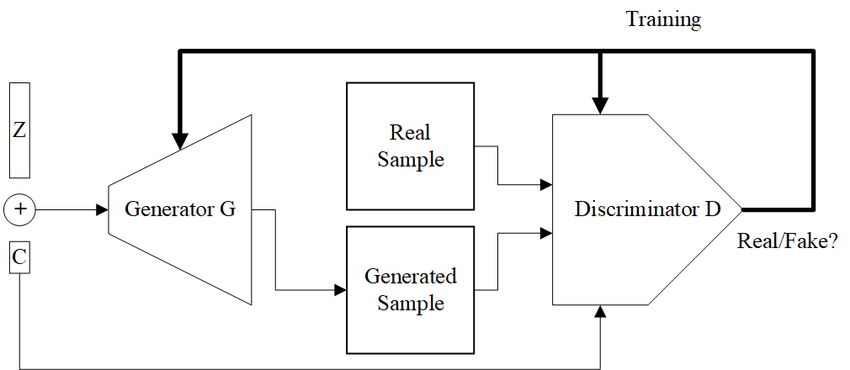
\includegraphics[width=1.0\linewidth]{GANS.png} % Corrected file name
        
    \end{figure}
\end{frame}

\begin{frame}
\frametitle{Methodology}
\framesubtitle{Model Architecture}
\begin{table}[ht]
    \centering
    \begin{tabular}{|p{0.45\textwidth}|p{0.45\textwidth}|}
        \hline
        \textbf{Generator Network} & \textbf{Discriminator Network} \\
        \hline
        
        Translate synthetic images into realistic images. & Differentiate between real images and generated images. \\
        \hline
        
        Several convolutional layers to process and transform input synthetic images. & Several convolutional layers to extract features from input images. \\
        \hline
        
        Maintain the integrity of image features. & Evaluates image in smaller patches for fine-grained details. \\
        \hline
        
        Techniques like batch normalization to stabilize and accelerate training. & Allows a small gradient when the unit is not active for training stability. \\
        \hline
    \end{tabular}
    % \caption{Comparison between Generator Network and Discriminator Network}
    \label{tab:gen_vs_disc}
    \end{table}

\end{frame}

\begin{frame}[t]
    \frametitle{Methodology}
    \framesubtitle{Models Declaration}
    The ConStructS model is a significant development in translating medical images without matched pairs.
    \vspace{0.3cm}
    \begin{itemize}
        \item <1-> \textbf{Contrastive learning:} A technique that helps keep important details in images by comparing similar and different parts of the input and output images
        \vspace{0.3cm}
        \begin{itemize}
            \item The goal is to bring similar examples (positive pairs) closer in the representation space and push dissimilar examples (negative pairs) further apart
        \end{itemize}
        \vspace{0.3cm}
        \item <2-> \textbf{Multi-Scale Structural Similarity (MS-SSIM):} A method that ensures the overall structure of images stays consistent across different sizes and resolutions
        \vspace{0.2cm}
        \begin{itemize}
            \item  measures the similarity between two images based on their structural content
        \end{itemize}
    \end{itemize}
\end{frame}

\begin{frame}[t]
    \frametitle{Methodology}
    \framesubtitle{Loss Functions}

    \begin{itemize}
        \item \textbf{Adversarial Loss}
        \begin{itemize}
            \item Trains both generator and discriminator networks.
            \item Generator produces images to fool the discriminator.
            \item Discriminator distinguishes real from generated images.
        \end{itemize}
    \end{itemize}

    \begin{block}{Adversarial Loss Formula}
    \small
    For the generator \(G\) and the discriminator \(D\):
    \[
    L_{GAN}(G,D) = E_{y \sim p_{data}(y)} [\log D(y)] + E_{x \sim p_{data}(x)} [\log (1 - D(G(x)))]
    \]
    \vspace{-0.6cm}
    \begin{itemize}
        \item \(E_{y \sim p_{data}(y)}\): Expected value over real images.
        \item \(E_{x \sim p_{data}(x)}\): Expected value over generated images.
        
    \end{itemize}
    \end{block}

\end{frame}

\begin{frame}[t]
    \frametitle{Methodology}
    \framesubtitle{Loss Functions}

    \begin{block}{discriminator's output for real data samples}
        \[
        E_{y \sim p_{data}(y)}[\log D(y)]
        \]
    \end{block}
    \vspace{0.6cm}
    
    \begin{itemize}
        \item \(y \sim p_{data}(y)\) means that \(y\) is sampled from the real data distribution.
        \vspace{0.6cm}
        \item \(\log D(y)\) is the logarithm of the probability that the discriminator assigns to \(y\) being a real sample.
    \end{itemize}

\end{frame}
\begin{frame}[t]
    \frametitle{Methodology}
    \framesubtitle{Loss Functions}

    \begin{block}{discriminator's output for fake data samples generated by generator}
        \[
        E_{x \sim p_{data}(x)}[\log (1 - D(G(x)))]
        \]
    \end{block}
    \vspace{0.6cm}
    
    \begin{itemize}
        \item \(x \sim p_{data}(x)\) means that \(x\) is sampled from the generator's input noise distribution.
        \vspace{0.6cm}
        \item \(G(x)\) is the generated data sample from the noise \(x\)
        \vspace{0.6cm}
        \item \(\log (1 - D(G(x)))\) is the logarithm of the probability that the discriminator assigns to \(G(x)\) being a fake sample.

    \end{itemize}

\end{frame}

\begin{frame}[t]
    \frametitle{Methodology}
    \framesubtitle{Loss Functions}
    \begin{itemize}
        \item <1-> \textbf{Role In training - Discriminator Training:}
        \begin{itemize}
            \item The discriminator \(D\) is trained to maximize this loss function
            \vspace{0.2cm}
            \item It tries to assign a high probability to real samples (\(D(y) \approx 1\)) and a low probability to fake samples (\(D(G(x)) \approx 0\)).
            \vspace{0.2cm}
            \item This part of the loss encourages \(D\) to become better at distinguishing between real and generated data.
 
        \end{itemize}
    \end{itemize}
    \begin{itemize}
        \item <2-> \textbf{Role In training - Generator Training:}
        \vspace{0.2cm}
        \begin{itemize}
             \item The generator \(G\) is trained to minimize this loss function
             \vspace{0.2cm}
             \item It tries to produce samples that \(D\) classifies as real (\(D(G(x)) \approx 1\)).
             \vspace{0.2cm}
             \item This part of the loss encourages \(G\) to generate more realistic data samples.
        \end{itemize}
    \end{itemize}
    
\end{frame}

\begin{frame}[t]
    \frametitle{Methodology}
    \framesubtitle{Loss Functions}
    \begin{itemize}
        \item \textbf{Objective of GANS}
        \vspace{0.4cm}
        \begin{itemize}
            \item The ultimate objective of a GAN is to reach a point where the discriminator cannot distinguish between real and generated data, i.e., \(D(y) = D(G(x)) = 0.5\)
            \vspace{0.4cm}
            \item At this point, the generator has learned to produce highly realistic data samples, and the discriminator is no better than random guessing
            \vspace{0.4cm}
            \item \textbf{Discriminator's Objective:} Maximize \(\log D(y) + \log (1 - D(G(x)))\)
            \vspace{0.4cm}
            \item \textbf{Generator's Objective:} Minimize \(\log (1 - D(G(x)))\)

        \end{itemize}
    \end{itemize}
    
\end{frame}

\begin{frame}[t]
    \frametitle{Methodology}
    \framesubtitle{Loss Functions}

    \begin{itemize}
        \item \textbf{Intuition}
         \vspace{0.4cm}
        \begin{itemize}
            \item \textbf{Discriminator:}
            \vspace{0.4cm}
            \begin{itemize}
                \item Wants to assign a high probability to real data (\(D(y) \rightarrow 1\)).
                \vspace{0.4cm}
                \item Wants to assign a low probability to generated data (\(D(G(z)) \rightarrow 0\)).
                \vspace{0.4cm}
            \end{itemize}
            
            \item \textbf{Generator:}
            \vspace{0.4cm}
            \begin{itemize}
                \item Wants to fool the discriminator by making \(D(G(z)) \rightarrow 1\), so that the generated data is classified as real.
            \end{itemize}
        \end{itemize}
    \end{itemize}

\end{frame}

\begin{frame}[t]
    \frametitle{Methodology}
    \framesubtitle{Loss Functions}

    \begin{itemize}
        \item \textbf{Binary Cross-Entropy Loss}: The forms $\log D(y)$ and $\log (1 - D(G(z)))$ correspond to the binary cross-entropy loss.
        \vspace{0.4cm}
        \item \textbf{Discriminator Loss} $L_D$:
        \vspace{0.4cm}
        \begin{block}{}
            \begin{equation}
                L_D = -\mathbb{E}_{y \sim p_{data}(y)} [\log D(y)] - \mathbb{E}_{x \sim p_z(z)} [\log (1 - D(G(z)))]
            \end{equation}
            \end{block}
            \vspace{0.4cm}
        \item \textbf{Generator Loss} $L_G$:
        \begin{block}{}
            \begin{equation}
                L_G = -\mathbb{E}_{x \sim p_z(z)} [\log D(G(z))]
            \end{equation}
            \end{block}


    \end{itemize}

\end{frame}

\begin{frame}[t]
    \frametitle{Methodology}
    \framesubtitle{Loss Functions}

    \begin{itemize}

        \item The original formulation as proposed by Goodfellow et al. in the GAN paper is often simplified for practical reasons, leading to the commonly used loss:
        \vspace{0.4cm}
        \begin{block}{}
            \begin{equation}
                L_{GAN}(G,D) = \mathbb{E}_{y \sim p_{data}(y)} [\log D(y)] + \mathbb{E}_{x \sim p_z(z)} [\log (1 - D(G(z)))]
            \end{equation}
            \end{block}
    \end{itemize}
    \footnotetext[1]{\url{https://arxiv.org/abs/1406.2661}}


\end{frame}



\begin{frame}[t]
    \frametitle{Methodology}
    \framesubtitle{Loss Functions}

    \begin{itemize}
        \item <1-> \textbf{Patch Constrastive Loss (PatchNCE)}
        \begin{itemize}
            \item Ensures semantic consistency by comparing patches of input and translated images
            \item Uses patches from the input and translated images to learn consistent feature representation
        
        \end{itemize}
        \item <2-> \textbf{Multi-Scale Structural Similarity (MS-SSIM) Loss}
        \begin{itemize}
            \item Maintains structural similarity at different image resolutions
            \item Measures the similarity between the input and translated images at different resolutions
        \end{itemize}
        \begin{block}{Note}<3->
            These loss functions collectively ensure that the generator produces high-quality, realistic, and semantically consistent images, while the discriminator continually improves its ability to distinguish between real and generated images
            \end{block}
    \end{itemize}
\end{frame}

\begin{frame}[t]
    \frametitle{Methodology}
    \framesubtitle{Performance}

    Performance of the generator and discriminator networks is regularly evaluated using the following metrics:

    \begin{itemize}
        \item \textbf{Pixel Accuracy}
        \begin{itemize}
            \item Indicates how well the generated images match the real images at the pixel level.
            \item Measures the proportion of correctly classified pixels in generated images compared to real images.
            \item Evaluates the fine detail replication in generated images.

        \end{itemize}
        \begin{block}{Pixel Accuracy Formula}
        \[
        \text{Pixel Accuracy} = \frac{\text{Number of Correctly Predicted Pixels}}{\text{Total Number of Pixels}}
        \]
        \end{block}
        A higher pixel accuracy indicates fewer discrepancies compared to real images at the pixel level.
    \end{itemize}
    
\end{frame}



\begin{frame}[t]
    \frametitle{Methodology}
    \framesubtitle{Performance}

    \begin{itemize}
        \item \textbf{Class Accuracy}
        \begin{itemize}
            \item Measures the accuracy of class-level classification in tasks like segmentation.
            \item Evaluates the ability to accurately reproduce different classes (e.g., organs, surgical tools). \\

        \end{itemize}
        \begin{block}{Class Accuracy Formula}
        \[
         \text{Class Accuracy} = \frac{\text{Number of Correctly Classified Pixels for a Class}}{\text{Total Number of Pixels in that Class}}
            \]
        \end{block}
        A high class accuracy indicates accurate representation of different classes as seen in real images.
    \end{itemize}
    
\end{frame}

\begin{frame}[t]
    \frametitle{Methodology}
    \framesubtitle{Performance}

    \begin{itemize}
        \item \textbf{CMean Intersection Over Union (mIOU)}
        \begin{itemize}
            \item Evaluates the overlap between predicted segmentation masks and ground truth masks.
            \item Provides a comprehensive measure of segmentation performance.

        \end{itemize}
        \begin{block}{Class Accuracy Formula}
        \[
    \text{IOU} = \frac{\text{Intersection Area}}{\text{Union Area}}
    \]
    \[
    \text{mIOU} = \frac{1}{N} \sum_{i=1}^{N} \text{IOU}_i
    \]
        \end{block}
        where \(N\) is the number of classes and \(\text{IOU}_i\) is the IOU for the \(i\)-th class. A higher mIOU indicates better segmentation performance.

    \end{itemize}
    
\end{frame}

\begin{frame}[t]
    \frametitle{Methodology}
    \framesubtitle{Performance}
Comparison with existing model(CycleGAN, GcGAN,LapMUNIT)
\vspace{0.2cm}
    \begin{itemize}
        \item <1-> \textbf{Enhanced Semantic Consistency}
        \vspace{0.2cm}
        \begin{itemize}
            \item Combines PatchNCE and MS-SSIM losses
            \vspace{0.2cm}
            \item Ensures both local and global semantic details are preserved
            \vspace{0.2cm}
        \end{itemize}
        \item <2-> \textbf{Improved Realism}
        \vspace{0.2cm}
        \begin{itemize}
            \item The combined loss functions generate realistic and structurally accurate images
            \vspace{0.2cm}
            \item Highly suitable for practical applications
            \vspace{0.2cm}

        \end{itemize}
        \item <3-> \textbf{Practical Utility}
        \vspace{0.2cm}
        \begin{itemize}
            \item Superior performance in downstream tasks such as segmentation
            \vspace{0.2cm}
            \item Highlight key phrases in bold or color to emphasize important points
            \vspace{0.2cm}
        \end{itemize}

    \end{itemize}
    
\end{frame}

\begin{frame}
    \frametitle{Evaluation and Results}
    \begin{itemize}
        \item \textbf{CycleGAN}: Effective for general tasks but struggles with semantic consistency in complex medical images
        \item \textbf{CcGAN} :Maintains geometric consistency but less effective in preserving fine details
        \item  \textbf{DRIT++:} Produces diverse outputs but may not maintain semantic consistency
        \item \textbf{LapMUNIT:}Designed for medical imaging, preserves structure but is computationally intensive
        \item  \textbf{SRUNIT}: Improved consistency but requires fine-tuning for complex datasets
        \item  \textbf{CUT} : Maintains local details but less effective globally
    \end{itemize}
    \begin{block}{Note}
        ConStructS shows superior performance in pixel accuracy, class accuracy, and mIOU compared to these baseline methods
        \end{block}
    
\end{frame}

\begin{frame}
    \frametitle{Evaluation and Results}
    \begin{itemize}
        \item Evaluation of the models
    \end{itemize}
    % Evaluation content here
    \begin{figure}
        \centering
        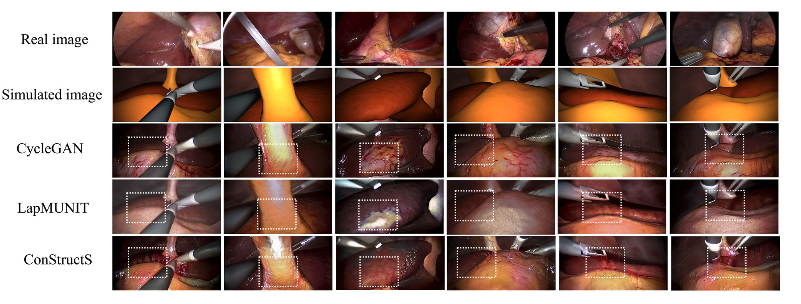
\includegraphics[width=1.0\linewidth]{eval.png} % Corrected file name
        
    \end{figure}
\end{frame}

\begin{frame}
    \frametitle{Evaluation and Results}
    \begin{itemize}
        \item Evaluation of the models with simulated image
    \end{itemize}
    % Evaluation content here
    \begin{figure}
        \centering
        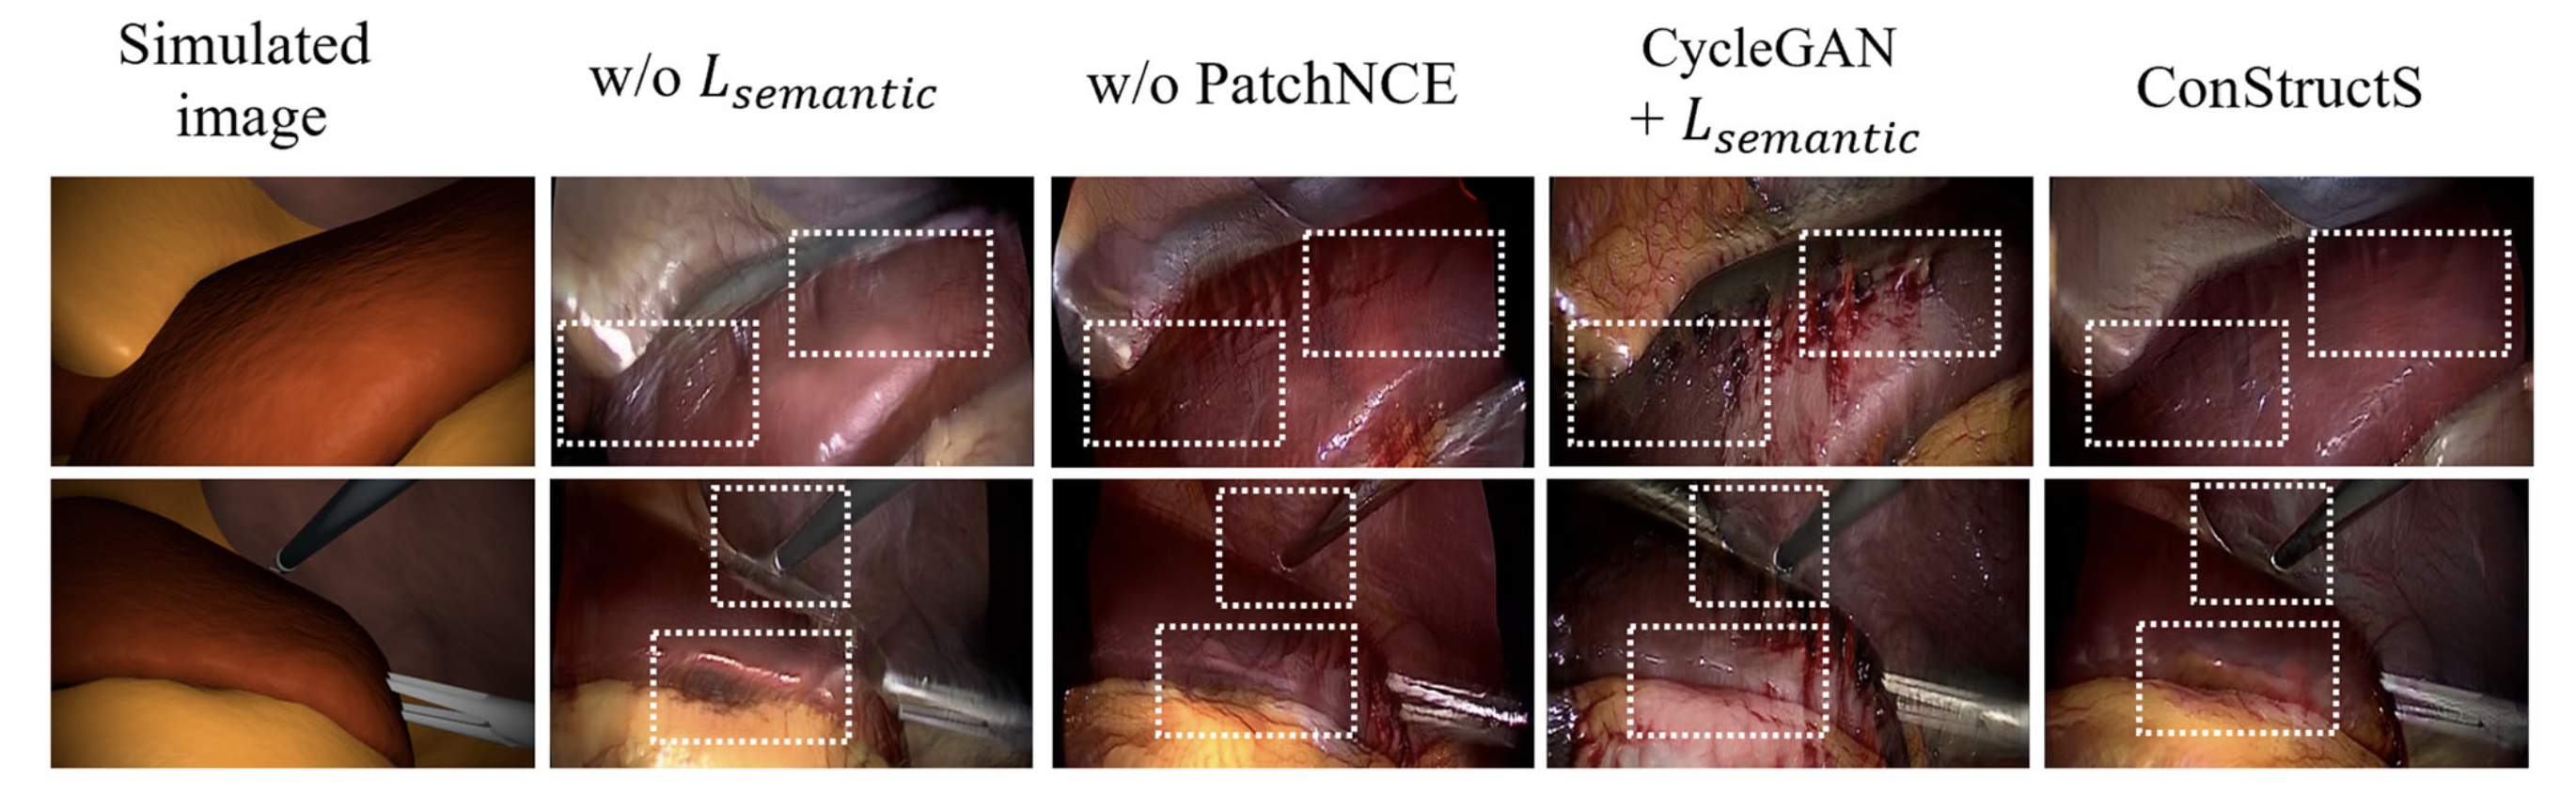
\includegraphics[width=1.0\linewidth]{result.png} % Corrected file name
        
    \end{figure}
\end{frame}



\begin{frame}
    \frametitle{Evaluation and Results(Model Comparison)}
    
    \begin{table}[ht]
     \tiny
    \centering
    \begin{tabular}{l l c c c}
    \toprule
    \textbf{Approach} & \textbf{Method} & \textbf{pxAcc} & \textbf{clsAcc} & \textbf{mIOU} \\
    \midrule
    Cycle consistency & CycleGAN  & 0.49 $\pm$ 0.08 & 0.41 $\pm$ 0.14 & 0.23 $\pm$ 0.09 \\
    & CycleGAN+VGG  & 0.52 $\pm$ 0.09 & 0.43 $\pm$ 0.11 & 0.25 $\pm$ 0.10 \\
    & DRIT++  & 0.42 $\pm$ 0.03 & 0.28 $\pm$ 0.05 & 0.17 $\pm$ 0.04 \\
    & LapMUNIT  & 0.53 $\pm$ 0.06 & 0.38 $\pm$ 0.08 & 0.25 $\pm$ 0.06 \\
    & UGAT-IT  & 0.50 $\pm$ 0.07 & 0.29 $\pm$ 0.07 & 0.19 $\pm$ 0.05 \\
    \midrule
    One-sided translation & GeGAN  & 0.51 $\pm$ 0.08 & \underline{0.44 $\pm$ 0.10} & 0.26 $\pm$ 0.08 \\
    & DistGAN  & 0.40 $\pm$ 0.03 & 0.28 $\pm$ 0.50 & 0.16 $\pm$ 0.04 \\
    \midrule
    Contrastive learning & SRC  & 0.51 $\pm$ 0.07 & 0.43 $\pm$ 0.16 & 0.25 $\pm$ 0.09 \\
    & NEGcut  & 0.53 $\pm$ 0.08 & 0.40 $\pm$ 0.12 & 0.24 $\pm$ 0.09 \\
    & FeSim  & 0.41 $\pm$ 0.10 & 0.38 $\pm$ 0.09 & 0.24 $\pm$ 0.09 \\
    & LeSim  & 0.44 $\pm$ 0.10 & 0.43 $\pm$ 0.09 & 0.24 $\pm$ 0.09 \\
    \midrule
    Semantic consistency & CycleGAN+SCC  & 0.50 $\pm$ 0.10 & 0.38 $\pm$ 0.12 & 0.25 $\pm$ 0.10 \\
    & CUT+SCC  & 0.42 $\pm$ 0.06 & 0.35 $\pm$ 0.12 & 0.18 $\pm$ 0.07 \\
    & SRUNIT  & 0.50 $\pm$ 0.08 & 0.30 $\pm$ 0.13 & 0.23 $\pm$ 0.08 \\
    \midrule
    Ablation study & ConStructS w/o $L_{semantic}$  & 0.50 $\pm$ 0.07 & 0.40 $\pm$ 0.14 & 0.26 $\pm$ 0.09 \\
    & ConStructS w/o PatchNCE  & 0.50 $\pm$ 0.10 & 0.40 $\pm$ 0.15 & 0.25 $\pm$ 0.10 \\
    & CycleGAN + $L_{semantic}$  & 0.49 $\pm$ 0.10 & 0.43 $\pm$ 0.15 & 0.24 $\pm$ 0.09 \\
    & \textbf{ConStructS}  & \textbf{0.59 $\pm$ 0.07} & \underline{0.44 $\pm$ 0.12} & \textbf{0.29 $\pm$ 0.09} \\
    \bottomrule
    \end{tabular}
    % \caption{The best result is indicated in \textbf{bold}, and the second best is \underline{underlined}.}
    \label{tab:model_comparison}
    \end{table}
    
\end{frame}



\begin{frame}
    \frametitle{Evaluation and Results}
    \begin{itemize}
        \item Best way
    \end{itemize}
    % Evaluation content here
    \begin{figure}
        \centering
        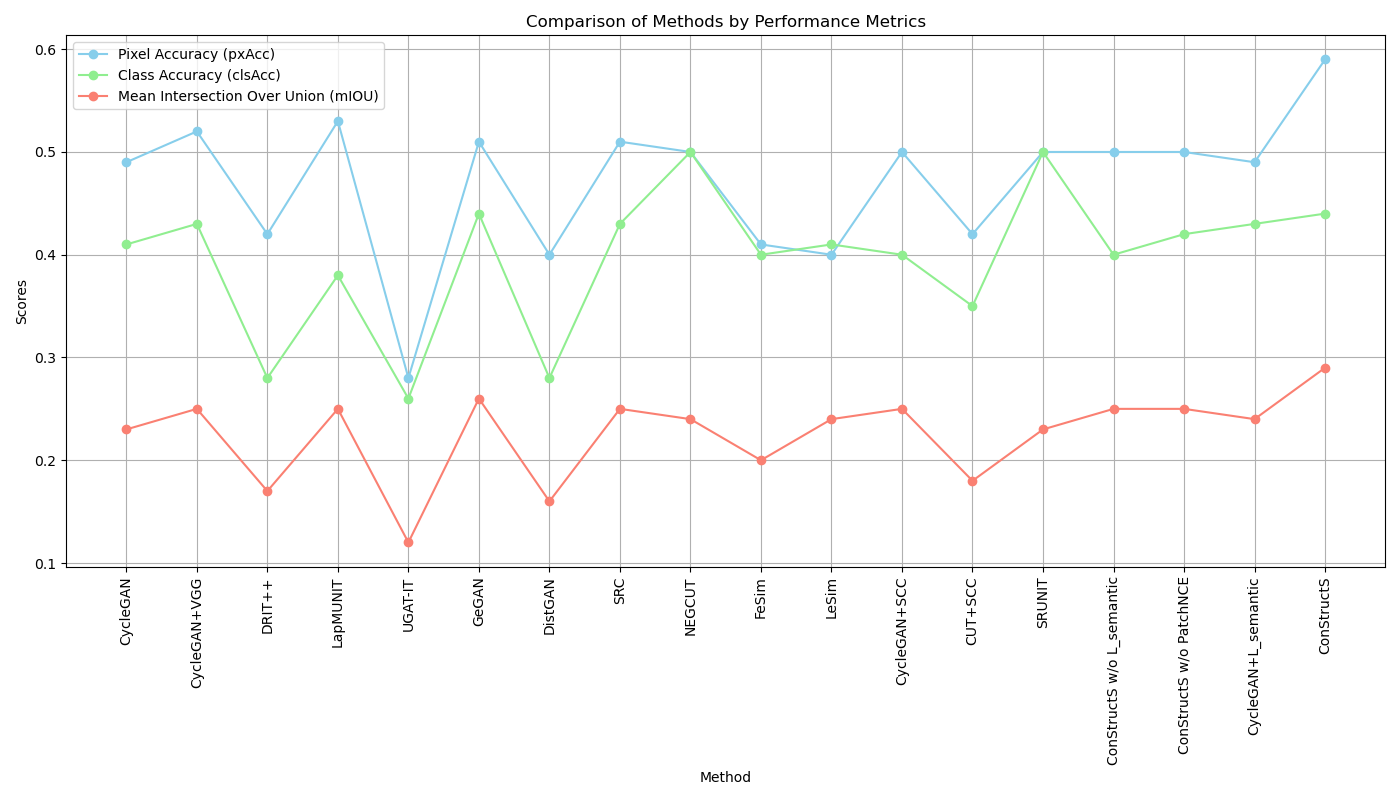
\includegraphics[width=0.8\linewidth]{model_eval.png} 
        
    \end{figure}
\end{frame}

\begin{frame}
    \frametitle{Evaluation and Results}
    \begin{itemize}
        \item \textbf{Summary }
        \vspace{0.2cm}
        \begin{itemize}
            \item <1-> CycleGAN is effective for general image translation tasks but struggles with maintaining semantic consistency and structural details compared to ConStructS, showing lower performance with pixel accuracy of 0.49, class accuracy of 0.41, and mIOU of 0.23
            \vspace{0.1cm}
            \item <2-> LapMUNIT, designed for medical imaging, preserves structural integrity but has moderate performance with lower class accuracy, achieving pixel accuracy of 0.53, class accuracy of 0.38, and mIOU of 0.25
            \vspace{0.1cm} 
            \item <3-> SRC, a contrastive learning method, provides a good balance of pixel and class accuracy but falls short in segmentation performance, with pixel accuracy of 0.51, class accuracy of 0.43, and mIOU of 0.25
            \vspace{0.1cm}
            \item <4-> SRUNIT, focused on semantic consistency, improves class accuracy but has lower mIOU, resulting in pixel accuracy of 0.50, class accuracy of 0.50, and mIOU of 0.23
            \vspace{0.1cm}
        \end{itemize}
    \end{itemize}
    % Evaluation content here
    
\end{frame}

\begin{frame}
    \frametitle{Evaluation and Results}
    \begin{itemize}
        \item \textbf{Summary of ConStructS Advantages }
        \vspace{0.2cm}
        \begin{itemize}
            \item <1-> Demonstrates superior ability to generate images that closely match real ones at the pixel level
            \vspace{0.2cm}
            \item <2-> Ensures accurate identification of different regions and objects within the images
            \vspace{0.2cm}
            \item <3-> Provides the best overlap between predicted and ground truth segmentation masks, indicating excellent segmentation performance
            \vspace{0.2cm}
            \item <4-> ConStructS outperforms all other models in maintaining semantic consistency and structural integrity across various metrics
            \vspace{0.2cm}
        \end{itemize}
    \end{itemize}
    % Evaluation content here
    
\end{frame}

\begin{frame}
    \frametitle{Evaluation and Results}
    \begin{itemize}
        \item <1-> \textbf{Analysis of Outliers, Anomalies and Variability }
        \vspace{0.2cm}
        \begin{itemize}
            
            \item Some generated images may show significant deviations from expected results, which can be identified as outliers. These outliers could include images where the translation fails to maintain semantic consistency or introduces artifacts
            \vspace{0.2cm}
        \end{itemize}
        \item <2-> \textbf{Potential Explanations}
        \vspace{0.2cm}
        \begin{itemize}
            \item Poor quality or insufficient diversity in the training data can lead to outliers
            \vspace{0.2cm}
            \item The architecture or training procedure might not fully capture all necessary features, leading to occasional failures in generating realistic images
            \vspace{0.2cm}
            \item Medical images can have complex and varied structures
        \end{itemize}
    \end{itemize}
    % Evaluation content here
    
\end{frame}

\begin{frame}
    \frametitle{Evaluation and Results}
    \vspace{0.2cm}
    \begin{itemize}
        \item <1-> \textbf{Variability }
        \vspace{0.2cm}
        \begin{itemize}
            \item The variability in model performance across different datasets indicates that the model's effectiveness can depend heavily on the specific characteristics of the data
            \vspace{0.2cm}
        \end{itemize}
        \item <2-> \textbf{Factors Contributing}
        \vspace{0.2cm}
        \begin{itemize}
            \item  Greater diversity in training data can lead to more robust models that generalize better across different datasets
            \vspace{0.2cm}
            \item  Some models may overfit to specific datasets and perform poorly on others, indicating limited generalization ability
            \vspace{0.2cm}
            \item  Variability in lighting, texture, and anatomical differences across datasets can affect performance
        \end{itemize}
    \end{itemize}
    % Evaluation content here
    
\end{frame}

\begin{frame}
    \frametitle{Evaluation and Results}
    \begin{itemize}
        \item \textbf{Uncertainty}
        \vspace{0.2cm}
        \begin{itemize}
            \item <1-> The inherent randomness in model training, such as weight initialization and data shuffling, can introduce variability in the results
            \vspace{0.2cm}
            \item <2-> Differences in evaluation metrics and their sensitivity to various aspects of image quality can also contribute to uncertainty
            \vspace{0.2cm}
            \item <3-> Uncertainty can lead to inconsistent performance across different runs or datasets, making it challenging to predict model behavior reliably
            \vspace{0.2cm}
            \item <4-> Understanding and mitigating these uncertainties is crucial for improving the robustness and reliability of the model
            \vspace{0.2cm}
            \item <5-> Affects the predictability and reliability of model performance
        \end{itemize}
    \end{itemize}
    % Evaluation content here
    
\end{frame}

\begin{frame}
    \frametitle{Evaluation and Results}
    \begin{itemize}
        \item \textbf{Practical Implimentation and Applications- Medical Image Analysis}
        \vspace{0.2cm}
        \begin{itemize}
            \item <1-> The ConStructS method can generate high-quality, annotated datasets from synthetic images, which are essential for training AI models used in medical image analysis
            \vspace{0.2cm}
            \item <2-> Improved segmentation models can assist in accurately identifying anatomical structures and abnormalities, enhancing diagnostic accuracy
            \vspace{0.2cm}
            \item <3-> Surgeons can use realistic, annotated images generated by ConStructS for virtual training and simulation, improving their skills without risking patient safety
            \vspace{0.2cm}
            \item <4-> Enhanced image translation can aid in creating detailed 3D models of patient anatomy, assisting surgeons in preoperative planning
            \vspace{0.2cm}
            \item <5-> High-quality image translation can enable more accurate remote diagnostics
        \end{itemize}
    \end{itemize}
    % Evaluation content here
    
\end{frame}

\begin{frame}
    \frametitle{Evaluation and Results}
    \begin{itemize}
        \item \textbf{Challenges}
        \vspace{0.2cm}
        \begin{itemize}
            \item <1-> \textbf{High Processing Power:} The ConStructS method requires significant computational resources for training, which might be a barrier for some institutions
            \vspace{0.2cm}
            \item <2-> Ensuring high-quality synthetic data is crucial
            \vspace{0.2cm}
            \item <3-> The model might need further tuning and validation to generalize effectively across different medical imaging. Common modalities include X-ray, CT (Computed Tomography), MRI (Magnetic Resonance Imaging), and Ultrasound
            \vspace{0.2cm}
            \item <4-> Deploying AI models in clinical settings requires navigating complex regulatory approval processes, which can be time-consuming and costly
            \vspace{0.2cm}
            \item <5-> Ensuring patient privacy and data security is paramount
        \end{itemize}
    \end{itemize}
    % Evaluation content here
    
\end{frame}

\begin{frame}
    \frametitle{Evaluation and Results}
    \vspace{0.2cm}
    \begin{itemize}
        \item \textbf{Opportunities}
        \begin{itemize}
            \item <1-> Ongoing research can further enhance the ConStructS method, making it more efficient and effective
            \vspace{0.2cm}
            \item <2-> Collaborations between research institutions can facilitate data sharing, leading to more diverse and comprehensive datasets for training
            \vspace{0.2cm}
            \item <3-> Combining ConStructS with other AI and machine learning techniques can lead to even more powerful tools for medical image analysis and diagnostics
            \vspace{0.2cm}
            \item <4-> The ConStructS method can be adapted for use in veterinary medicine, improving diagnostics and treatment planning for animals
            \vspace{0.2cm}
            \item <5-> Beyond healthcare, the method can be applied to other fields requiring high-quality image translation, such as autonomous driving and satellite imagery analysis
        \end{itemize}
    \end{itemize}
    % Evaluation content here
    
\end{frame}


\begin{frame}
\frametitle{Summary and Conclusion}

\textbf{Summary of Key Findings}
\vspace{0.2cm}
\begin{itemize}
    \item <1-> The ConStructS method significantly outperformed other models in key metrics
    \vspace{0.2cm}
    \item <2-> It demonstrates its superior ability to produce realistic and semantically consistent medical images
    \vspace{0.2cm}
    \item <3-> The integration of PatchNCE and MS-SSIM losses in ConStructS proved to be highly effective
    \vspace{0.2cm}
    \item <4-> ConStructS showed consistent performance across different datasets, indicating its robustness and generalization capability
    \vspace{0.2cm}
    \item <5-> This study identified potential outliers and variability in the results, primarily due to differences in data quality and the inherent complexity of medical images
    \vspace{0.2cm}
    \item <6-> These applications highlight the practical utility and broad impact of the ConStructS method in the medical field
\end{itemize}
% Conclusion content here
\end{frame}

\begin{frame}
    \frametitle{Summary and Conclusion}
    \textbf{Future Outlook}
    \vspace{0.2cm}
    \begin{itemize}
       \item <1-> Further research is needed to improve the ConStructS method's ability to generalize across different medical imaging modalities, such as X-ray, MRI, and CT scans
       \vspace{0.2cm}
       \item <2-> Future research should focus on creating and using datasets that cover a wide variety of medical conditions, anatomical structures, and patient demographics
       \vspace{0.2cm}
       \item <3-> Exploring ways to optimize the ConStructS model for real-time applications in clinical settings
       \vspace{0.2cm}
       \item <4-> Investigating how ConStructS can be integrated with other AI technologies, such as reinforcement learning and natural language processing
       \vspace{0.2cm}
       \item <5-> For example, combining image translation with automated diagnosis systems could significantly enhance clinical decision-making
    \end{itemize}
    % Conclusion content here
    \end{frame}

\begin{frame}
        \frametitle{Summary and Conclusion}
        \textbf{Unsolved Questions}
        \vspace{0.2cm}
        \begin{itemize}
            \item <1-> \textbf{Optimal Training Techniques}
            \vspace{0.2cm}
            \begin{itemize}
                \item What are the most effective training techniques to ensure consistent performance across different medical imaging modalities?
                \vspace{0.2cm}
                \item Further research is needed to identify the best practices for training models like ConStructS on varied datasets
                \vspace{0.2cm}
            \end{itemize}
            \item <2-> \textbf{Handling Extreme Variability}
            \vspace{0.2cm}
            \begin{itemize}
                \item How can the model be adapted to handle extreme variability in patient anatomy and medical conditions?
                \vspace{0.2cm}
                \item This remains a critical challenge, as medical images can vary widely across different populations and health scenarios
                \vspace{0.2cm}
            \end{itemize}
            \item <3-> Temporal information from patient scans taken over time could enhance the accuracy and reliability of image translations
            
        \end{itemize}
        % Conclusion content here
\end{frame}

\begin{frame}
    \frametitle{Summary and Conclusion}
    \textbf{Future Research Directions}
    
    \begin{itemize}
        \item <1-> \textbf{Exploring Advanced Architectures}
        
        \begin{itemize}
            \item Future research should explore advanced neural network architectures, such as transformers, to further enhance the performance of ConStructS
            
            \item These architectures have shown promise in other domains and could be beneficial for medical image translation
            \vspace{0.2cm}
        \end{itemize}
        \item <2-> \textbf{Open Data Sharing}
        
        \begin{itemize}
            \item Promoting collaborative research initiatives and open data sharing among medical institutions and researchers can accelerate advancements in the field
            \vspace{0.2cm}
        \end{itemize}
        \item <3-> \textbf{Regulatory and Ethical Frameworks}
        
        \begin{itemize}
            \item This includes ensuring patient privacy, data security, and addressing any biases in the model training process
            \vspace{0.2cm}
        \end{itemize}
        \item <4-> Conducting extensive clinical trials and real-world validations to assess the practical utility and safety of the ConStructS method
    
    \end{itemize}
    % Conclusion content here
\end{frame}

\begin{frame}
    \frametitle{Summary and Conclusion}
    \textbf{Conclusion}
    \begin{itemize}
        \item <1-> ConStructS is a significant advancement in unpaired image translation for medical applications
        \item <2-> Combines contrastive learning and multi-scale structural similarity to maintain semantic consistency and structural integrity
        \item <3-> Demonstrates superior performance with higher pixel accuracy, class accuracy, and mIOU
        \item <4-> Generates high-quality, annotated medical images valuable for AI model training, surgical planning, and telemedicine
        \item <5-> Highlights future research areas like tuning and validation across different imaging modalities
        \item <6-> Aims to enhance model generalization and robustness across varied patient demographics
    \end{itemize}
    % Conclusion content here
\end{frame}


\begin{frame}
\frametitle{The End}
\begin{center}
\scalebox{2}{Further Questions?}
\end{center}
\end{frame}

\begin{frame}
    \frametitle{Buffer Slides}
    \textbf{Patch-based Contrastive Learning}
    \begin{itemize}
        \item Instead of applying contrastive learning at the image level, it is applied at the patch level.
        \item This means the image is divided into patches, and the contrastive loss is computed for each patch.
        \item The PatchNCE loss is calculated by summing the InfoNCE loss over multiple layers and spatial locations:
        \begin{block}{}
            \[
            L_{\text{PatchNCE}} = \mathbb{E}_{x \sim X} \sum_{l=1}^{L} \sum_{s=1}^{S} L_{\text{NCE}}
            \]
        \end{block}
        Here, $L$ is the number of layers, and $S$ is the number of spatial locations.
    \end{itemize}
    
\end{frame}

\begin{frame}
    \frametitle{Buffer Slides}
    \textbf{Multi-Scale Structural Similarity (MS-SSIM)}
    \begin{itemize}
        \item MS-SSIM (Multi-Scale Structural Similarity) is an extension of the Structural Similarity (SSIM) index, which measures the similarity between two images based on their structural content
        \item MS-SSIM evaluates similarity at multiple scales, making it more robust to variations in image resolution and structural details.
        \begin{block}{}
            \begin{center}
            MS-SSIM$(x, y) = \prod_{i=1}^{M} (\text{SSIM}_i(x, y))^{W_i}$
            \end{center}
            \end{block}
            This weighted combination ensures that structural similarity is assessed at different resolutions, capturing both fine and coarse details.

    \end{itemize}
    
\end{frame}

\begin{frame}
    \frametitle{Buffer Slides}
    \textbf{Combination}
    \begin{itemize}
        \item Ensures that the translated images are indistinguishable from real images.
        \item Preserves local features by enforcing consistency in patch representations.
        \item Maintains structural consistency across multiple scales, ensuring the translated images retain the structural integrity of the original images.
        \item Overall Loss Function :
        
\begin{block}{}
    \begin{center}
    $L_{\text{total}} = L_{\text{GAN}} + \lambda_x L_{\text{PatchNCE}}(X) + \lambda_y L_{\text{PatchNCE}}(Y) + \lambda_{ss} L_{\text{semantic}}$
    \end{center}
    \end{block}
    Here, $\lambda_x$, $\lambda_y$, and $\lambda_{ss}$ are weights for the PatchNCE and semantic losses.

        
    \end{itemize}
    
\end{frame}



\end{document}
